\documentclass[11pt]{article} 
\usepackage[utf8]{inputenc}

\usepackage{geometry} 
\geometry{a4paper}
\usepackage{url}
\usepackage{graphicx} 
\usepackage{booktabs} 
\usepackage{array} 
\usepackage{paralist} 
\usepackage{verbatim} 
\usepackage{subfig} 
\usepackage{amsmath}
\usepackage{fancyhdr} 
\pagestyle{fancy} 
\renewcommand{\headrulewidth}{0pt} 
\lhead{}\chead{}\rhead{}
\lfoot{}\cfoot{\thepage}\rfoot{}


\usepackage{sectsty}
\allsectionsfont{\sffamily\mdseries\upshape}


\usepackage[nottoc,notlof,notlot]{tocbibind} 
\usepackage[titles,subfigure]{tocloft} 
\renewcommand{\cftsecfont}{\rmfamily\mdseries\upshape}
\renewcommand{\cftsecpagefont}{\rmfamily\mdseries\upshape} 



\title{Notes on Fracture - Cubic Law and Linear Law}
\author{Ivan Marin}
\date{\today} 

\begin{document}
\maketitle


\section{Cubic Law}
\subsection{Deduction from Navier-Stokes}
This model of the fracture assumes that the flow is viscous and slow, so the inertia terms in the Navier-Stokes can be neglected. The fracture is saturated with water, and are thin.
\subsection{Cubic Law for Discharge}
The cubic law for discharge in the direction of the fracture is 
\begin{align}
Q_{s}(s) = -\beta^{*}b^{3}\frac{\partial \tilde{\phi(s)}}{\partial s}
\end{align}
where b is the total aperture of the fracture and $\beta^{*}$ is equal to
\begin{align}
\beta^{*} = \frac{\rho g}{12\mu}
\end{align}
where $\rho$ is the density of water, $[kg/m^{3}]$; $g$ is the gravity acceleration $[m^{2}/s]$, and $\mu$ is the dynamic viscosity, $[Pa.s]$, $[kg/(m.s^{2})]$. 

\subsection{Cubic Law for the Potential}
\begin{align}
Q_{s}(s) = - \frac{\beta^{*}b^{3}}{k}\frac{\partial \Phi}{\partial s}
\end{align}

\section{Linear Law}
\subsection{Linear Law Approximations}
The Linear Law for flow in the fractures assumes that the fracture is filled with a material of hydraulic conductivity $k^{*}$, that the flow is viscous and slow and incompressible.
\subsection{Linear Law for Discharge}
The discharge is equal to 
\begin{align}
Q_{s}(s) = - k^{*}b\frac{\partial \tilde{\phi(s)}}{\partial s}
\end{align}

\subsection{Linear Law for Potential}
\begin{align}
Q_{s}(s) = \frac{k^{*}b}{k}\frac{\partial \Phi}{\partial s}
\end{align}

%\begin{figure}
%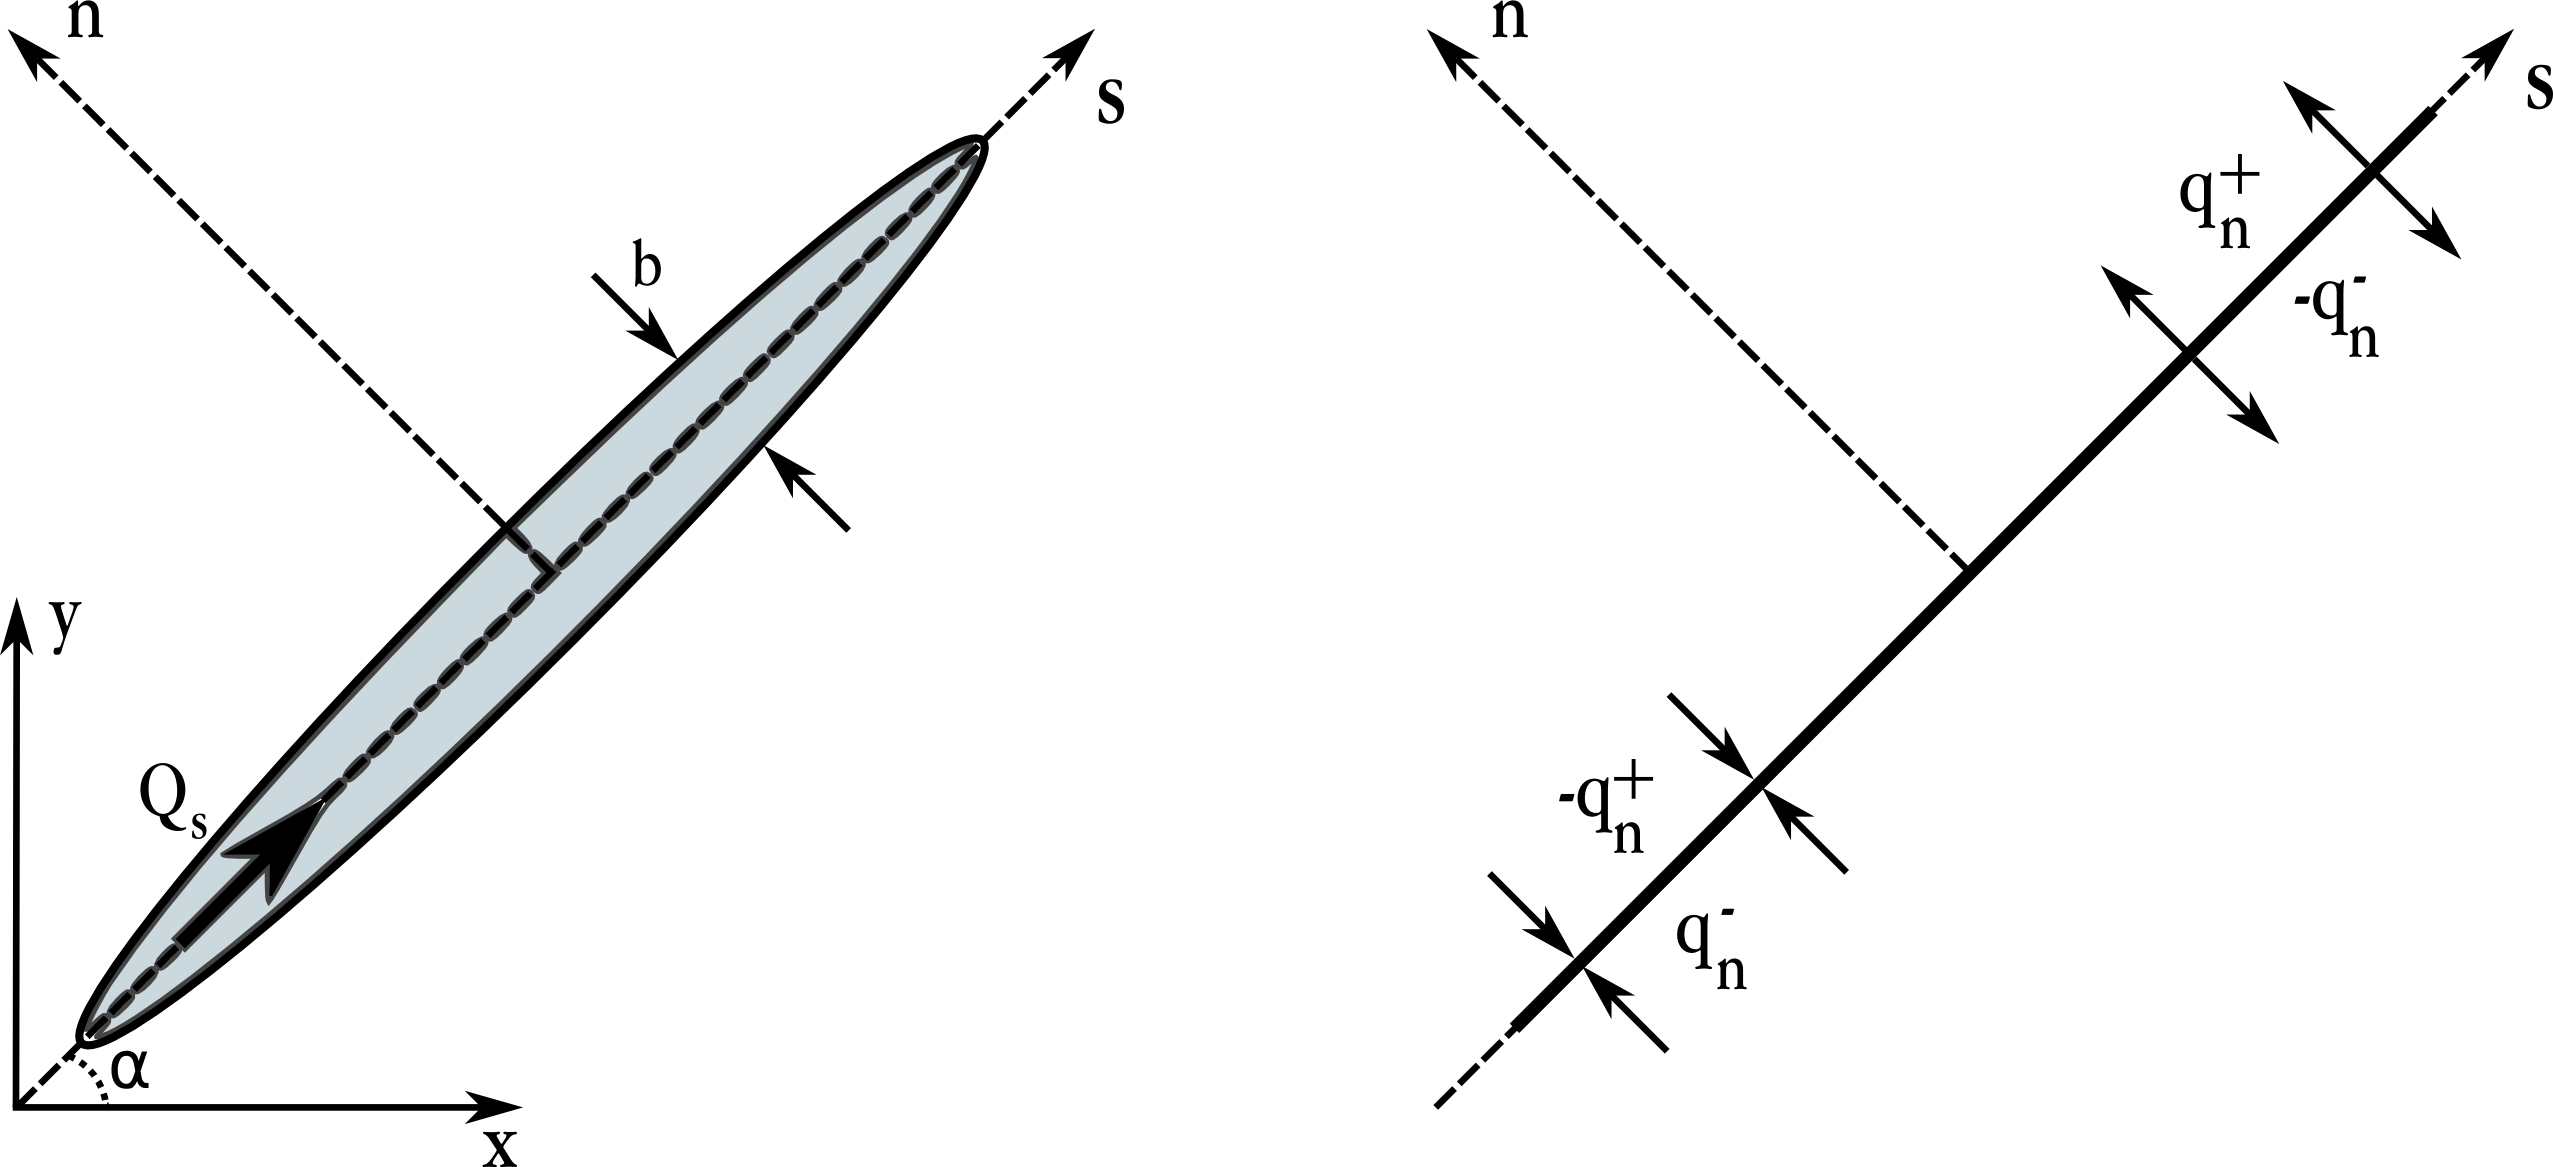
\includegraphics[width = 8cm]{img/esquema_frac.png}
%\end{figure}
%\begin{figure}
%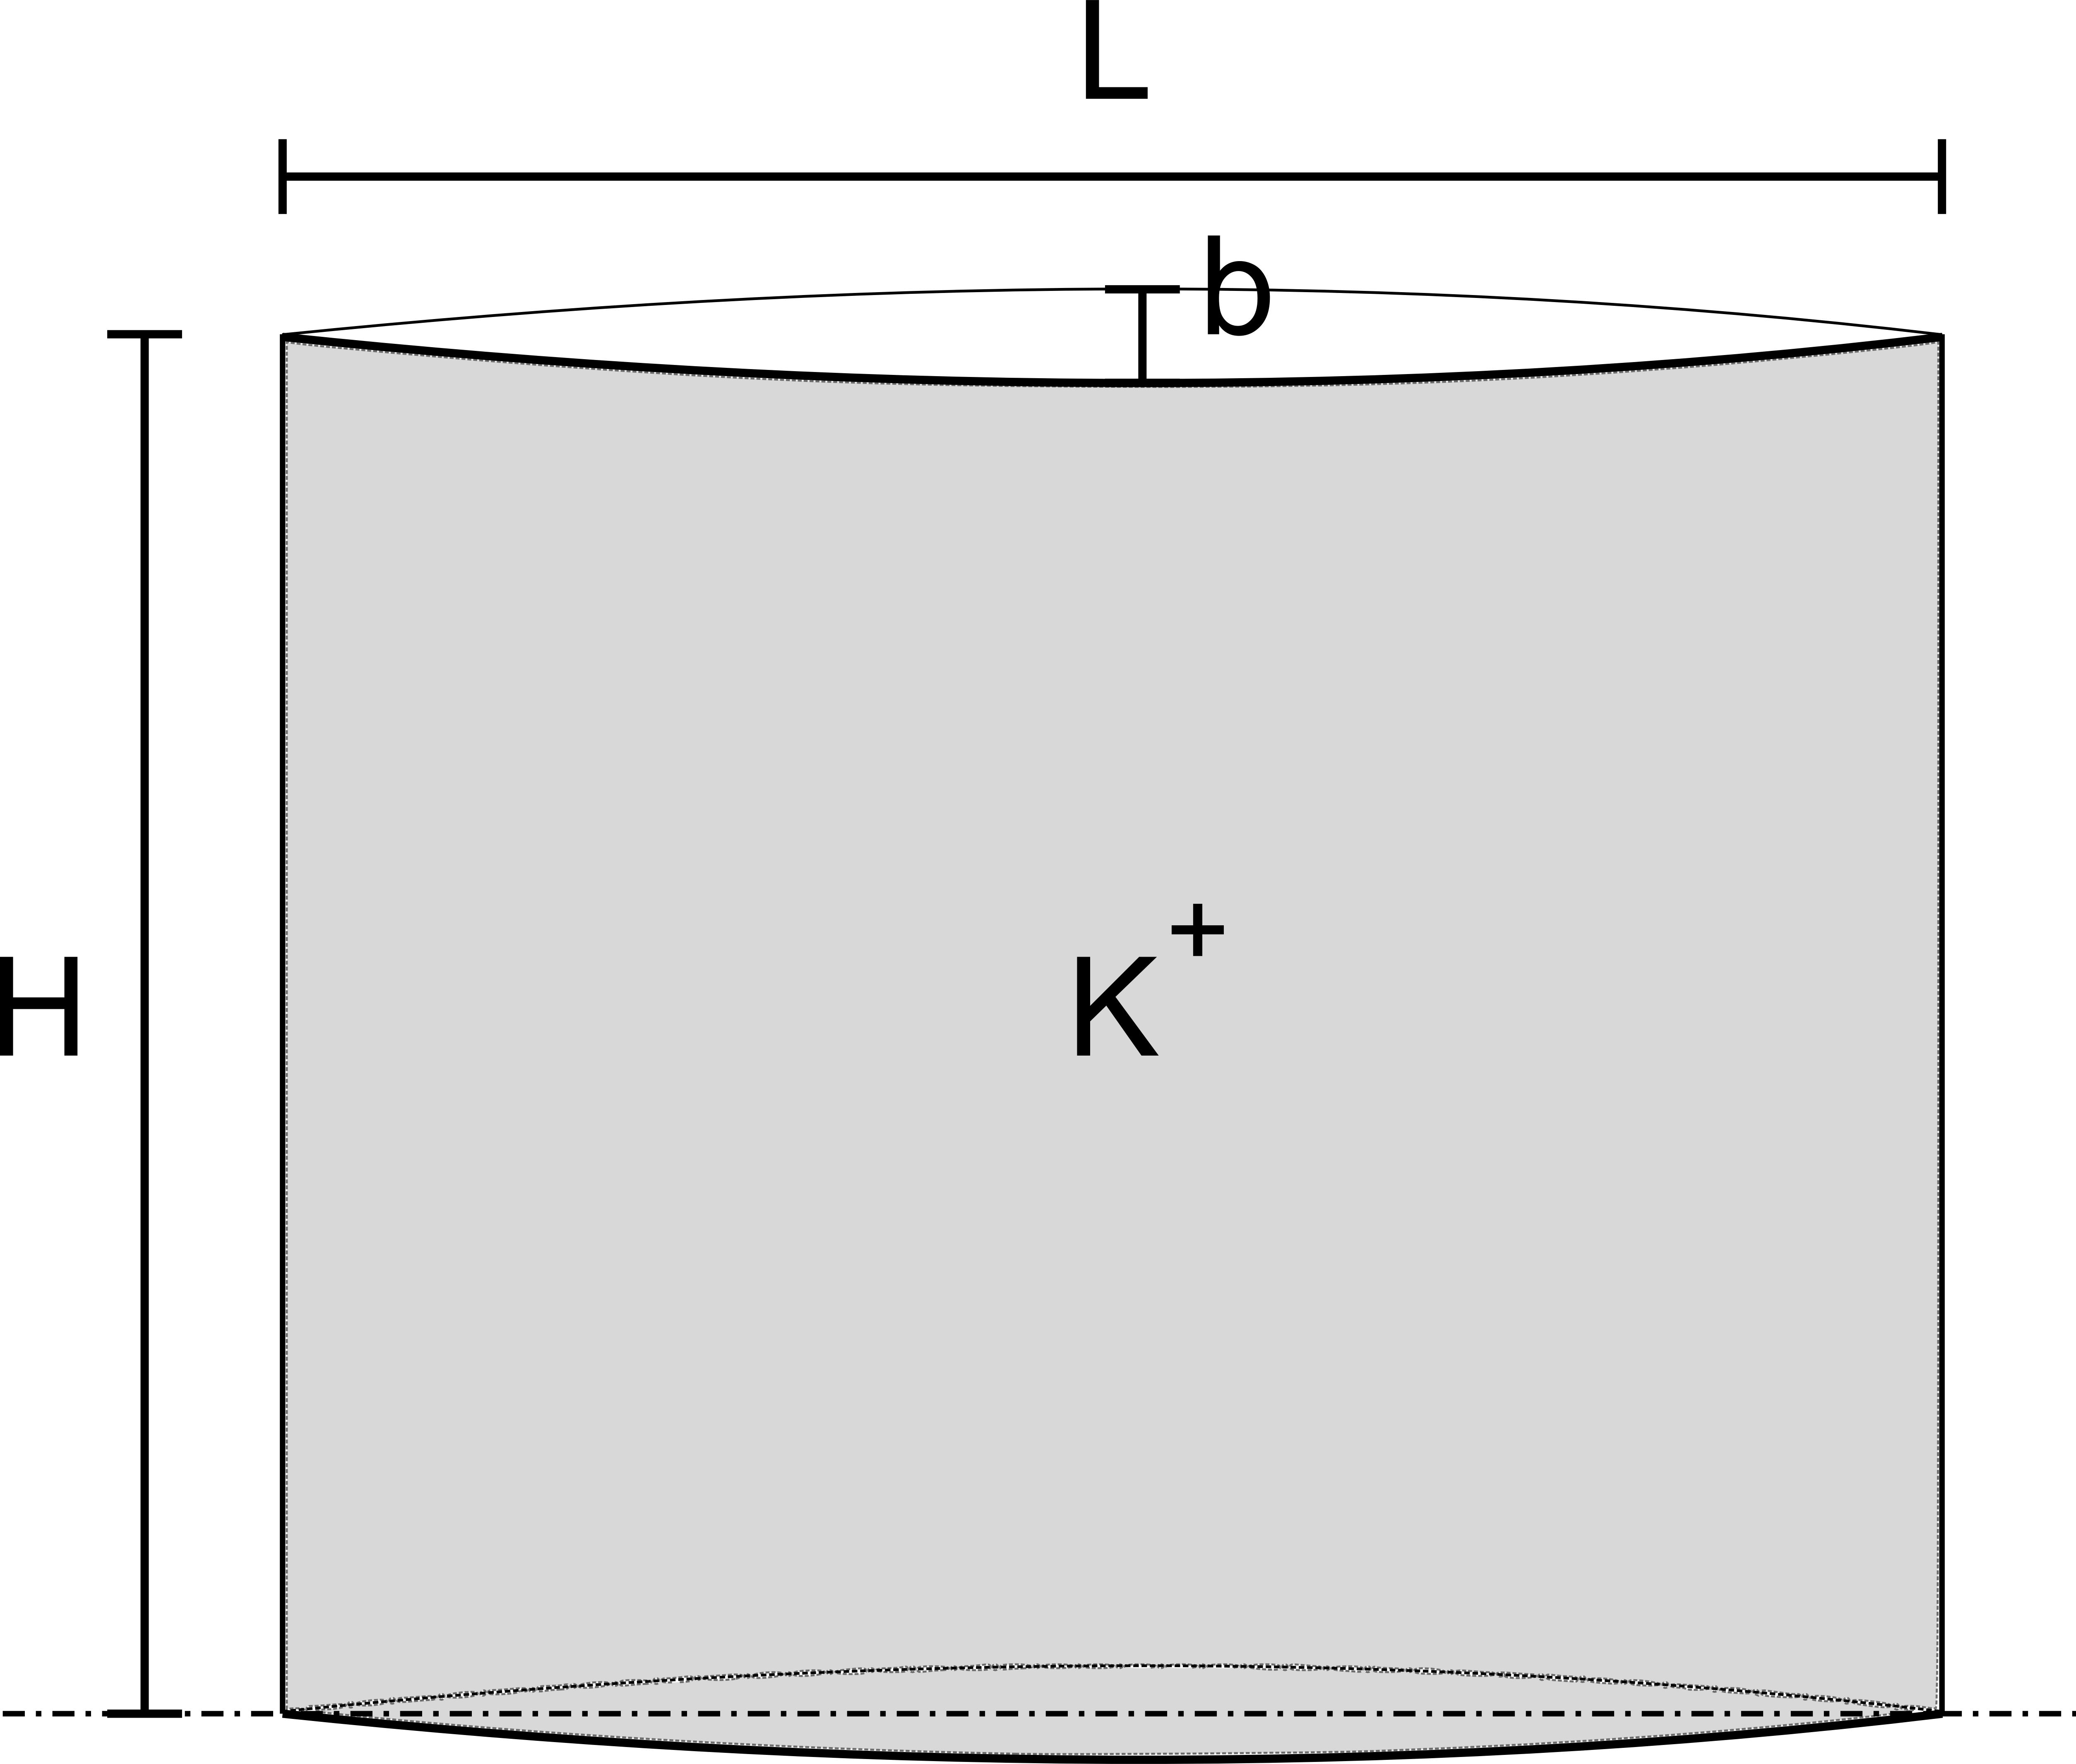
\includegraphics[width = 8cm]{img/frac_elip.png}
%\end{figure}



\end{document}